\documentclass{article}
\usepackage[ruled, linesnumbered]{algorithm2e}
\def\showtopic{Finite Difference Method}
\def\showtitle{Lab 2: Oliker--Pr\"ussner Method\\ Solving Alexandroff Solution for Monge--Amp\`ere Equation}
\def\showabs{Lab 1}
\def\showauthor{Ting Lin, 1700010644}
\def\showchead{LIN}
\usepackage{amsmath, amsfonts, amsthm}

\usepackage{graphicx, epstopdf}
\usepackage{color}
\usepackage{geometry, graphicx}
\usepackage{algorithm, algorithmic}
\usepackage{bm}
\usepackage{multirow}
\usepackage{ulem}
\geometry{left = 5em, right = 5em}
\usepackage{listings}
\usepackage{xcolor}
%% notation macro
\newcommand{\F}{\mathcal F}
\newcommand{\T}{\mathcal T}
\newcommand{\I}{\mathcal I}
\newcommand{\U}{\mathcal U}
\newcommand{\R}{\mathbb R}
\renewcommand{\P}{\mathcal P}
\newcommand{\uP}{ \mathcal \uline P}
\newcommand{\B}{\mathcal B}
%\newcommand{\R}{\mathbb R^2}
\newcommand{\Z}{\mathbb Z}
\newcommand{\C}{\mathbb C}
\newcommand{\laplacian}{\triangle}
\newcommand{\grad}{\nabla}
\renewcommand{\div}{\textrm{div~}}

\newcommand{\diff}[2]{\frac{\partial #1}{\partial #2}}
\newcommand{\difff}[3]{\frac{\parial #1^2}{\partial #2 \partial #3}}
\newcommand{\diFF}[2]{\frac{\partial #1^2}{\partial^2 #2}}
\newcommand{\diam}{\text{ diam }}
%% non-noation macro
\newcommand{\IN}{\text{  in  }}
\newcommand{\ON}{\text{  on  }}
\newcommand{\st}{\text{s.t.  }}
\newcommand{\tbc}{{\color{red}[TBC]}}
\renewcommand{\Return}{\textbf{return~}}
\newcommand{\Break}{\textbf{break~}}
\newcommand{\Continue}{\textbf{continue~}}
\renewcommand{\And}{\textbf{~and~}}
\newcommand{\Or}{\textbf{~or~}}
%% enviorment
\newtheorem{proposition}{Proposition}
\newtheorem{definition}{Definition}
\newtheorem{corollary}{Corollary}
\newtheorem{remark}{Remark}

\DeclareMathOperator{\argmin}{arg~min}

\renewcommand{\algorithmicrequire}{ \textbf{Input:}} %Use Input in the format of Algorithm
\renewcommand{\algorithmicensure}{ \textbf{Output:}} %UseOutput in the format of Algorithm
\title{\textbf{\showtitle}}
\author{\showauthor}
\usepackage{indentfirst}
\usepackage{fancyhdr}  
\pagestyle{fancy}
\lhead{\textbf {\showtopic} }
\chead{\showchead} 
\rhead{\textbf {\showabs} }
\lfoot{} 
\cfoot{\thepage}
\rfoot{} 
\renewcommand{\headrulewidth}{0.4pt} 
\DeclareMathOperator{\size}{size}
\DeclareMathOperator{\maxd}{\max\nolimits^\delta}
\DeclareMathOperator{\nhi}{\mathcal N_h^{I}}
\DeclareMathOperator{\nhp}{\mathcal N_h^{\partial}}
\DeclareMathOperator{\mind}{\min\nolimits^\delta}
\DeclareMathOperator{\MA}{MA}
\DeclareMathOperator{\MAJ}{MAJ}
\newcommand{\bV}{\mathbb V}
\begin{document}
	\maketitle
	\thispagestyle{fancy}
	\tableofcontents
	
	\section*{}

\section{Problem Setting and Finite Difference}
\subsection{Monge--Amp\`ere Equation}
We solve the following Monge--Amp\`ere Equation in 2D. 
\begin{align}
\det(D^2u) = f & \IN \Omega\\ 
u|_{\partial \Omega} = g & \ON \partial \Omega
\end{align}
Define the subgradient of a convex function $u$ on some interior point $x$:
$$\partial u(x) = \{p \in \R^2|u(y) \le u(x) + p\cdot (y-x) \text{ for all } y\}.$$
The alexandroff solution satisfies 
$$|\partial u| = f$$
for all interior points. The concept can be generalized to the case when $f$ is a measure, means 
$$|\cup_{x\in E}\partial u(x)| = |f(E)|$$

For $f>0$, we can show the existence and uniqueness of Alexandroff solution. Moreover, the Alexandroff solution and the viscosity solution are the same. We omit these concept and only call the solution of MA equation hereafter.

\subsection{Oliker--Pr\"ussner Method}
For nodal function $u_h$ on point set $X_h = \{x_i\}$, the OP method seek for a solution 
\begin{align}
|\partial u_h(x_i)| = f_h(x_i) & x_i \in \nhi\\ 
u|_{\partial \Omega} = g_h(x_i) & x_i \in \nhp
\end{align}
Here the subgradient of a nodal function is defined as 
$$\partial u_h(x_i) = \{p \in \R^2|u_h(x_j) \le u_h(x_i) + p\cdot (x_j-x_i) \text{ for all } x_j\}.$$
We now bridge the connection between subgradients that of function and nodal function. Consider the convex envelope 
$$\Gamma u_h(x) =  \sup\{L(x): L \text{ is affine and } L(x_i) \le u_h(x_i)\}.$$
A nodal function is convex if and only if $u_h(x_i) = \Gamma u_h(x_i)$.
The connection is 
\begin{proposition}
	$$\partial u_h(x_i) = \partial \Gamma u_h(x_i).$$
\end{proposition}
The existence of OP solution is guaranteed by Perron's iteration. Suppose we have a good initial value such that $u_h^0(x_i) = g_h(x_i)$ for $x_i \in \nhp$ and $|\partial u_h^0(x_i)| \ge x_i$ for $x_i \in \nhi$. Then consider the following algorithm:
\begin{algorithm}[H]
	\caption{Framework of Perron's Iteration}
	\label{alg:1}
	\begin{algorithmic}[1]
		\WHILE{not converge}
		\FOR{$x_i \in \nhi$}
		\STATE Find $u$ such that $|\partial \tilde u_h(x_i)| = f_h(x_i)$, where $\tilde u_h$ modify the value of $u_h$ at $x_i$ to $u$.
		\STATE Update $U_h(x_i) = u$.
		\ENDFOR
		\ENDWHILE
	\end{algorithmic}
\end{algorithm}
Algorithm~\ref{alg:1} generates a sequence $u_h^k$, we can prove the following things by induction and the monotonicity of subgradient. 
\begin{proposition}
	$u_h^{k+1}(x_i) \ge u_h^{k}(x_i)$, and each $u_h^k$ is convex. Moreover, 	$$|\partial \tilde u_h^k(x_i)| \ge f_h(x_i)$$
\end{proposition}
After this, the existence of OP solution is clear: Since $u_h^k$ is convex, we have $$u_h(x_i) \le  \sup\{L(x): L \text{ is affine and } L(x_i) \le u_h(x_i) \text{ for all } x_i \in nhp\}.$$
Hence $u_h^k(x_i)$ is bounded and increasing thus convergent. Denote the limit as $u_h^{\infty}(x_i)$, argument based on continuous dependency yields that $u_h^{\infty}$ is our desired OP solution. In practice we choose the convergence criterion as $u_h^{k}(x_i) < u_h^{k-1}(x_i) + tol$ for all interior points.

\subsection{Computations of subgradient}
However, the subgradient is not computable, hence we need a little more work to derive our algorithm. Consider a convex nodal function $u_h$. Since $\Gamma u_h$ is clearly piecewise linear function, thus we can define a mesh $\T$ such that the Lagrange interpolation of $u_h(x_i)$ under $\T$ is exactly $\Gamma u_h$:
$$\I_{\T}u_h(x) = \Gamma u_h(x).$$
We call $\T$ be the induced mesh of $u_h$. The key point is that 
\begin{proposition}
	Suppose $u_h$ is convex. Then $\T$ is the induced mesh if and only if $\I_{\T}u_h$ is convex.
\end{proposition}
\begin{proof}
	Clearly $\Gamma u_h$ has the following equivalent definition:
	$$\Gamma u_h(x_i) =  \sup\{~\I_{\T}u_h(x): \T \text{ over all possible mesh }\}.$$
	We only need to verify that $\I_{\T}u_h(x_i) \ge \Gamma u_h(x_i)$. Since for any simplex $T \in \T'$ containing $x_i$, the convexity of $\I_{\T}u_h$ yields that $\I_{\T'}u_h(x_i) \le \I_{\T}u_h(x_i)$. Take supremum on $\T'$ we conclude the result.
\end{proof}
Notice that $\I_{\T}u_h$ is equivalent to all jump of interior face $F = T^+ \cap T^-$:
$$[\I_{\T}u_h]_F = -(\grad \I_{\T}u_h)|_{T^+}\cdot \textbf{n}^+ -(\grad \I_{\T}u_h)|_{T^-}\cdot \textbf{n}^-$$
is nonnegative. This will be a good criterion in practice to check whether $\T$ is the induced mesh. The computation of subgradient are made easy once the induced mesh is obtained, according to the following proposition.
\begin{figure}[H]
	
	
	\centering
	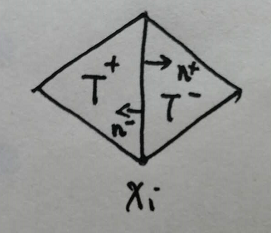
\includegraphics[scale=0.4]{../fig/jump.png}
	\caption{Jump of an edge}
	\label{fig:jump}
\end{figure}

\begin{proposition}
	Suppose $u_h$ is convex and $\T$ is its induced mesh. Then the subgradient of $u_h(x_i)$ is the area of
	$$ConvexHull( \{\grad \I_{\T}u_h: x_i \text{ is attached to} T \in \T.\}.)$$
	Moreover, if we swap all $T$ around $x_i$ clockwisely, then the gradient we obtained is clockwise. Moreover, all gradient lie in the convex hull. Hence the convex hull is obtained automatically.
\end{proposition}

\section{Implementation Details}
In this section we deal with two issues. The first is how to get a suitable initial value (together with the initial induced mesh). The second is how to update the value in perron's iteration and update the induced mesh. We first introduce the data structure used in implementation.

\subsection{Data Structure}
\textbf{X,Y} : $N$ array, stores the position of nodes.

\textbf{U}: $N$ array, stores the value of nodes.

\textbf{G}: $N$ array, stores the exact solution (and boundary value therefore) of nodes.

\textbf{F}: $N$ array, stores RHS.

\textbf{elem}: $NT\times 3$ array, stores which three nodes form an element. (in counterclockwise order as usual).


\textbf{adj}: (adjacent linked list)$N \times 40 \times 3$ array, stores the elements around node $i$ (in clockwise order). Here we use array to simulate the linked list since many operation we encounter is add and delete. Each $adj(i,:,:)$ is a linked list, with $adj(i,x,1)$ is the corresponding element, $adj(i,x,2)$ indicates the location in element, i.e. satisfying the equation 
$$elem(adj(i,x,1),adj(i,x,2)) = i$$
and $adj(i,x,3)$ indicates the entry next to x in the linked list.

\textbf{elemind}: (element indexs) $NT\times 3$ array. $elemind(T,i)$ tells us where $T$ is on the linked list $adj(i,:,:)$.

\textbf{bdadj}: $N\times 2$. For boundary points, $bdadj(i,1), bdadj(i,2)$ is the neighborhood of $i$. Used in lifting the boundary.

~~
~~


Here are several comments.

1. From only one \textbf{elem} array, we can recover all the auxiliary arrays, the implementation is in \textbf{meshinit.m} and we omit it here.

2. There are slight difference of adjacent linked list for interior point and boundary point. The former is looped while thee latter is not. However the implementation will treat both as looped linked list, and once we need lift the boundary value (as we will see), we need to drop the virtual link by some special judge. (See Figure~\ref{fig:all} )

\begin{figure}[H]


	\centering
	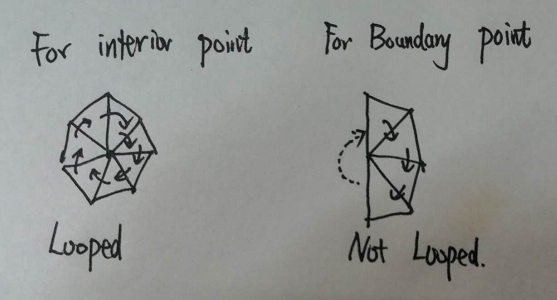
\includegraphics[scale=0.3]{../fig/adjlinkedlist.png}
		\caption{Linked list for interior point and boundary point.}
			\label{fig:all}
\end{figure}

\subsection{Mesh Flipping}
In this subsection we deal with how to get the induced mesh if we lift value at $x_i$. When lifting $x_i$, two kinds of edge will change their jump value.  1) edges adjacent to $x_i$; 2) edges opposite to $x_i$. The next result shows we only need to consider the adjacent ones.

\begin{figure}[H]
	
	
	\centering
	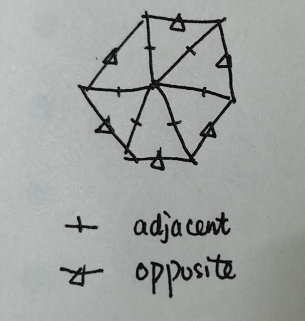
\includegraphics[scale=0.3]{../fig/adjopp.png}
	\caption{Two kinds of edges around $x_i$}
	\label{fig:adjopp}
\end{figure}
\begin{proposition}
	\label{prop:flip-th}
	Suppose $u_h$ is convex and $\T$ is its induced map. Suppose $F$ is opposite to $x_i$, then $[\I_{\T}u_h]_F$ is increasing w.r.t $x_i$. Suppose $F$ is adjacent tto $x_i$, then $[\I_{\T}u_h]_F$ is decreasing w.r.t $x_i$.
\end{proposition}
\begin{proof}
	WLOG we assume $ABC,ABD$ is two elements, with $A=(-1,0), B = (1,0), C = (x_1,y_1), D = (x_2, -y_2)$, where $y_1, y_2 > 0$. Then the jump is $u_h(C)/y_1 + u_h(D)/y_2$, increasing w.r.t two opposite nodes. The second statement can be proved in a similar way.
\end{proof}

Hence we only need to consider the adjacent edges. For each adjacent edge $F_t$, suppose $F_t = T_{t} \cap T_{t+1}$. We first notice that since $(\grad \I_{\T}u_h)|_{T_{t}}$ is linear on $u_h(x_i)$, we can find $P_t, Q_t \in \R^2$ such that $(\grad \I_{\T}u_h)|_{T_{t}} = P_t - u_h(x_i)Q_t$. Suppose the normal vector of $F_t$ on $T_t$ is $N_t$, then the jump is 
$$P_t\cdot N_t- u_h(x_i)Q_t\cdot N_t - P_{t+1}\cdot N_{t+1} + u_h(x_i)Q_{t+1}\cdot N_{t+1}.$$ 

By Proposition~\ref{prop:flip-th}, we know if $u_h(x_i) \le \theta_t$, then $[\I_{\T}u_h]_{F_t} \le 0$. Here 
\begin{equation}
\label{eq:th}
\theta_t = \frac{P_t\cdot N_t - P_{t+1}\cdot N_{t+1}}{Q_t\cdot N_t -Q_{t+1}\cdot N_{t+1} }.
\end{equation}
Hence $u_h(x_i) = U_i$ makes $|\partial u_h(x_i)| = f_h(x_i)$. We conclude that if $U_i < \min_t \theta_t$ then we can use the current $\T$ to compute subgradient. Otherwise we should flip the edge $t_0 := \argmin \theta_t$, and recalculate all things around $x_i$. 

\begin{figure}[H]
	
	
	\centering
	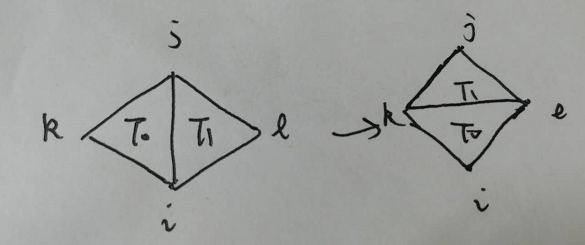
\includegraphics[scale=0.3]{../fig/flip.png}
	\caption{Edge flipping}
	\label{fig:flip}
\end{figure}
The flip procedure is simple (see Figure~\ref{fig:flip}): we just change $elem(T_0,:)$ and $elem(T_1,:)$, then update the adjacent linked list about $i,j,k,l$. At last we update the $elemind$ array. It is noticeable that flipping has very nice property.

\begin{proposition}
	Suppose $u_h(x_i) = \theta_{t_0}$ and we have flipped the edge $F_{t_0} = T_0 \cap T_1$ into $F' = T_0' \cap T_1'$. Then the jump of other edges do not change, while the jump of new value is increasing w.r.t. $x_i$.
\end{proposition}
\begin{proof}
	The only thing need to verify is edge like $ik,lk,jk,lk$. This is because in the threshold, the values in $x_i, x_j, x_k, x_l$ are in the same plane. Hence the jump of $ik$, for example, will not change. The latter statement is because $F'$ is opposite to $x_i$.
\end{proof}

In practice, we use subfunction $getdis$ to compute $P_t, Q_t, N_t$. 

\subsection{Lift the Boundary}
Now we are ready to face the first problem: how to get a suitable initial value for Perron's iteration. We first choose 
$$u_h(x_i) = \frac{A}{2}(x_i)^2 - R^2$$
such that $u_h$ is negative on $\nhp$. The $A$ is chosen sufficiently large such that $|\partial u_h(x_i)| \ge f_h(x_i)$. We have proved that for the quadratic function, Delaunay triangulation gives the induced mesh $\T_0$. Thus we can compute the subgradient using $\T_0$ and then choose a suitable $A$. 

 Now we use following algorithm to lift the boundary value from $u_h(x_i)$ to $g_h(x_i)$, see Algorithm~\ref{alg:2}.
 
 
\begin{algorithm}[htbp]
	\caption{Lift the Boundary}
	\label{alg:2}
	\begin{algorithmic}[1]
		\STATE \textbf{inputs:} $u_h, g_h$.
		\WHILE{$\max_{x_i \in \nhp}g_h(x_i) - u_h(x_i) > tol$}
			\FOR{$x_i \in \nhp$}
			\IF{$g_h(x_i) - u_h(x_i) < tol$}
			\STATE \Continue
			\ENDIF
			\WHILE{true}
				\FOR{$t = 1:size(adj(x_i))+1$}
					\IF {$T_t$ and $T_{t+1}$ are not adjacent (the virtual link)}
						\STATE \Continue
					\ENDIF
					\STATE Compute $\theta_t$ by \eqref{eq:th}.
				\ENDFOR
				\STATE $t_0 = \argmin \theta_t$.
				\IF{$x_i$ is not corner point}
					\STATE $\theta_{bd} = \frac{1}{2}(u_h(x_j)+u_h(x_k))$ (average of two neighborhood).
					\ELSE
					\STATE $\theta_{bd} = \infty$
				\ENDIF
				\STATE $\theta_0 =\min(\theta_{t_0}, \theta_{bd})$
				\IF{$\theta_0 > g_h(x_i)$}
				\STATE $u_h(x_i):=g_h(x_i)$
				\STATE \Break
				\ENDIF
				\IF{$\theta_0 > \theta_{bd} - \varepsilon$}
				\STATE $u_h(x_i):=\theta_{bd}$
				\STATE \Break
				\ELSE{}
				\STATE Flip $F_{t_0}$
				\STATE $u_h(x_i) = \theta_0$.
				\STATE \Continue
				\ENDIF
		\ENDWHILE
		\ENDFOR

		\ENDWHILE
	\end{algorithmic}
\end{algorithm}

We now show the algorithm will stop and give the correct $u_h(x_i)$. The value of $u_h(x_i)$ will increase until either reaches $g_h(x_i)$$u_h$ is not convex at $x_i$. The only possible case is $u_h(x_i) = \theta_{bd}$. Thus each step we can lift $u_h(x_i)$ to $\min(g_h(x_i), \theta_{bd})$. 

Next we show for each step if we assign $u_h(x_i)$ to $\min(g_h(x_i), \theta_{bd})$, then it will converge. We have obtained a sequence $u_h^k(x_i)$, which is increasing and bounded. Thus it has a limit $v_h$.

\begin{proposition}
	$v_h(x_i) = g_h(x_i).$
\end{proposition}
\begin{proof}
	Routine argument gives us that if $x_j,x_k$ is the neighborhood of $x_i$, then $$v_h(x_i) = \min(g_h(x_i), \frac{1}{2}(v_h(x_j) + v_h(x_k))).$$
	For corner point, we certainly have $v_h(x_i) = g_h(x_i)$.
	Denote $S = \{i| v_h(x_i) = g_h(x_i)\}$.
	We prove by contradiction, suppose for some $x_i$, $v_h(x_i) < g_h(x_i)$, we choose $x_i$ such that $v_h(x_i)$ is smallest and the distance from $x_i$ to four corners is smallest. Then $v_h(x_i) = \frac{1}{2}(v_h(x_j) + v_h(x_k)))$ tells us that either $j$ or $k$ is in $S$. Suppose $j \in S$, then $k \notin S$, otherwise $v_h(x_i) \ge g_h(x_i)$. 
	
	Suppose $l_{-1} = j, l_0 = i, l_1 = k, \cdots, l_m$ are a series such that $l_i$ and $l_{i+1}$ are neighborhood, with $l_{-1}, l_m \in S$ while others $\notin S$. Then $$v_h(x_{l_{s}}) = \frac{1}{2}(v_h(x_{l_{s-1}}) + v_h(x_{l_{s+1}}))$$ for $s = 0,1,\cdots m-1$. Again we deduce that $v_h(x_i) \ge g_h(x_i)$ since $v_h$ is linear, $g_h$ is convex, with the same boundary value. Therefore all boundary points are in $S$.
\end{proof}

\subsection{Perron's Update}
We deal with Perron's update for some interior point $x_i$, notice that the area of subgradient is a piecewise quadratic function. We have the following algorithm, see Algorithm~\ref{alg:3}.
\begin{algorithm}[htbp]
	\caption{Perron's Update}
	\label{alg:3}
	\begin{algorithmic}[1]
		\STATE \textbf{inputs:} $u_h, f_h, x_i$.
		\WHILE{true}
		\FOR{$t = 1:size(adj(x_i))+1$}
		\IF {$T_t$ and $T_{t+1}$ are not adjacent (the virtual link)}
		\STATE \Continue
		\ENDIF
		\STATE Compute $\theta_t$ by \eqref{eq:th}.
		\ENDFOR
		\STATE $t_0 = \argmin \theta_t$.
		\IF{$subgrad(\theta_{t_0}) > f_h(x_i)$}
		\STATE Flip $F_{t_0}$
		\STATE $u_h(x_i):=\theta_{t_0}$
		\STATE \Continue
		\ELSE
		\STATE Compute $C = subgrad(u_h(x_i))/(u_h(x_i) - \theta_{t_0})^2$
		\STATE $u_h(x_i):= \theta_{t_0} - \sqrt{f_h(x_i)/C}$
		\ENDIF
		\ENDWHILE
	\end{algorithmic}
\end{algorithm}

Here subgrad is a function compute the area of polygon formed by all discrete gradient over $T_t$.

\section{Numerical Result}
In this section we test OP method for several result: 1)  smooth solution. 2) piecewise smooth solution. 3) Singular solution. Please see \textbf{loadfunction.m} for details.

We show the $L^\infty$ error and discrete $W_2^p$ error on $h = 1/2, 1/4, 1/8$, here the tolerance of both lift the boundary algorithm and Perron's iteration is chosen as $\varepsilon = 1e-10, 1e-6$, and the quadrate rule we use $quadpts(1)$ as low order and $quadpts(4)$ as high order. 
\subsection{tol = 1e-10, low order quadrate rule}
\begin{table}[H]
	\centering
	\caption{Problem 1}
	\begin{tabular}{|c|c|c|c|c|c|c|c|c|}
		\hline
		& iter  & time(s) & $L_{\infty}$ & order & $W_1^2$  & order & $W_2^2$  & order \\ \hline
		1   & 2     & 0.00    & 1.12E-01     & 0.00  & 6.15E-01 & 0.00  & 4.24E-01 & 0.00  \\ \hline
		1/2 & 568   & 0.06    & 4.78E-02     & 1.23  & 5.39E-01 & 0.19  & 3.42E-01 & 0.31  \\ \hline
		1/4 & 4093  & 2.16    & 1.37E-02     & 1.80  & 2.51E-01 & 1.10  & 1.66E-01 & 1.04  \\ \hline
		1/8 & 20428 & 48.53   & 3.55E-03     & 1.95  & 8.35E-02 & 1.59  & 5.66E-02 & 1.55  \\ \hline
	\end{tabular}
\end{table}
\begin{table}[H]
	\centering
	\caption{Problem 2}
	\begin{tabular}{|c|c|c|c|c|c|c|c|c|}
		\hline
		& iter  & time(s) & $L_{\infty}$ & order & $W_1^2$  & order & $W_2^2$  & order \\ \hline
		1   & 2     & 0.00    & 4.02E-01     & 0.00  & 2.20E+00 & 0.00  & 1.52E+00 & 0.00  \\ \hline
		1/2 & 326   & 0.04    & 4.19E-02     & 3.26  & 8.23E-01 & 1.42  & 5.83E-01 & 1.38  \\ \hline
		1/4 & 2196  & 1.20    & 2.90E-02     & 0.53  & 7.89E-01 & 0.06  & 6.21E-01 & -0.09 \\ \hline
		1/8 & 18374 & 44.43   & 1.27E-02     & 1.19  & 6.25E-01 & 0.34  & 5.04E-01 & 0.30  \\ \hline
	\end{tabular}
\end{table}
\begin{table}[H]
	\centering
	\caption{Problem 3}
	\begin{tabular}{|c|c|r|r|r|r|r|r|r|}
		\hline
		& iter  & \multicolumn{1}{c|}{time(s)} & \multicolumn{1}{c|}{$L_{\infty}$} & \multicolumn{1}{c|}{order} & \multicolumn{1}{c|}{$W_1^2$} & \multicolumn{1}{c|}{order} & \multicolumn{1}{c|}{$W_2^2$} & \multicolumn{1}{c|}{order} \\ \hline
		1   & 26    & 0.00                         & 8.58E-01                          & 0.00                       & 4.70E+00                     & 0.00                       & 3.24E+00                     & 0.00                       \\ \hline
		1/2 & 326   & 0.04                         & 2.37E-01                          & 1.86                       & 5.57E+00                     & -0.24                      & 3.66E+00                     & -0.17                      \\ \hline
		1/4 & 2196  & 1.42                         & 1.87E-01                          & 0.34                       & 5.61E+00                     & -0.01                      & 4.26E+00                     & -0.22                      \\ \hline
		1/8 & 18374 & 29.20                        & 8.54E-02                          & 1.13                       & 5.50E+00                     & 0.03                       & 4.77E+00                     & -0.16                      \\ \hline
	\end{tabular}
\end{table}


\subsection{tol = 1e-6, low order quadrate rule}
\begin{table}[H]
	\centering
	\caption{Problem 1}
	\begin{tabular}{|c|c|c|c|c|c|c|c|c|}
		\hline
		& iter & time(s) & $L_{\infty}$ & order & $W_1^2$  & order & $W_2^2$  & order \\ \hline
		1   & 2    & 0.00    & 1.12E-01     & 0.00  & 6.15E-01 & 0.00  & 4.24E-01 & 0.00  \\ \hline
		1/2 & 241  & 0.03    & 4.79E-02     & 1.23  & 5.40E-01 & 0.19  & 3.42E-01 & 0.31  \\ \hline
		1/4 & 911  & 0.63    & 1.41E-02     & 1.77  & 2.51E-01 & 1.10  & 1.66E-01 & 1.04  \\ \hline
		1/8 & 2614 & 9.41    & 4.27E-03     & 1.72  & 8.45E-02 & 1.57  & 5.65E-02 & 1.55  \\ \hline
	\end{tabular}
\end{table}

\begin{table}[H]
	\centering
	\caption{Problem 2}
	\begin{tabular}{|c|c|c|c|c|c|c|c|c|}
		\hline
		& iter & time(s) & $L_{\infty}$ & order & $W_1^2$  & order & $W_2^2$  & order \\ \hline
		1   & 2    & 0.00    & 4.02E-01     & 0.00  & 2.20E+00 & 0.00  & 1.52E+00 & 0.00  \\ \hline
		1/2 & 170  & 0.03    & 4.18E-02     & 3.26  & 8.23E-01 & 1.42  & 5.82E-01 & 1.38  \\ \hline
		1/4 & 949  & 0.70    & 2.91E-02     & 0.53  & 7.90E-01 & 0.06  & 6.21E-01 & -0.09 \\ \hline
		1/8 & 4149 & 13.37   & 1.35E-02     & 1.10  & 6.28E-01 & 0.33  & 5.06E-01 & 0.30  \\ \hline
	\end{tabular}
\end{table}

\begin{table}[H]
	\centering
	\caption{Problem 3}
	\begin{tabular}{|c|c|c|c|c|c|c|c|c|}
		\hline
		& iter & time(s) & $L_{\infty}$ & order & $W_1^2$  & order & $W_2^2$  & order \\ \hline
		1   & 15   & 0.00    & 8.58E-01     & 0.00  & 4.70E+00 & 0.00  & 3.24E+00 & 0.00  \\ \hline
		1/2 & 176  & 0.03    & 2.37E-01     & 1.86  & 5.57E+00 & -0.24 & 3.66E+00 & -0.17 \\ \hline
		1/4 & 841  & 0.66    & 1.86E-01     & 0.35  & 5.61E+00 & -0.01 & 4.26E+00 & -0.22 \\ \hline
		1/8 & 2196 & 8.25    & 8.49E-02     & 1.13  & 5.51E+00 & 0.03  & 4.77E+00 & -0.17 \\ \hline
	\end{tabular}
\end{table}
\subsection{tol = 1e-10, high order quadrate rule}
\begin{table}[H]
	\centering
	\caption{Problem 1}
	\begin{tabular}{|c|c|r|r|r|r|r|r|r|}
		\hline
		& iter  & \multicolumn{1}{c|}{time(s)} & \multicolumn{1}{c|}{$L_{\infty}$} & \multicolumn{1}{c|}{order} & \multicolumn{1}{c|}{$W_1^2$} & \multicolumn{1}{c|}{order} & \multicolumn{1}{c|}{$W_2^2$} & \multicolumn{1}{c|}{order} \\ \hline
		1   & 2     & 0.00                         & 8.10E-02                          & 0.00                       & 4.43E-01                     & 0.00                       & 3.06E-01                     & 0.00                       \\ \hline
		1/2 & 481   & 0.05                         & 2.59E-02                          & 1.64                       & 3.14E-01                     & 0.50                       & 2.04E-01                     & 0.58                       \\ \hline
		1/4 & 3268  & 1.89                         & 7.02E-03                          & 1.88                       & 1.43E-01                     & 1.13                       & 9.76E-02                     & 1.06                       \\ \hline
		1/8 & 17112 & 46.10                        & 1.79E-03                          & 1.97                       & 4.79E-02                     & 1.58                       & 3.35E-02                     & 1.54                       \\ \hline
	\end{tabular}
\end{table}

\begin{table}[H]
	\centering
	\caption{Problem 2}
	\begin{tabular}{|c|c|c|c|c|c|c|c|c|}
		\hline
		& iter  & time(s) & $L_{\infty}$ & order & $W_1^2$  & order & $W_2^2$  & order \\ \hline
		1   & 2     & 0.00    & 1.92E-01     & 0.00  & 1.05E+00 & 0.00  & 7.24E-01 & 0.00  \\ \hline
		1/2 & 369   & 0.04    & 3.50E-02     & 2.45  & 7.07E-01 & 0.57  & 4.63E-01 & 0.65  \\ \hline
		1/4 & 538   & 2.91    & 1.47E-02     & 1.25  & 3.95E-01 & 0.84  & 2.84E-01 & 0.70  \\ \hline
		1/8 & 97076 & 259.91  & 4.93E-03     & 1.58  & 3.01E-01 & 0.39  & 2.57E-01 & 0.15  \\ \hline
	\end{tabular}
\end{table}


\begin{table}[H]
	\centering
	\caption{Problem 3}
	\begin{tabular}{|c|c|c|c|c|c|c|c|c|}
		\hline
		& iter  & time(s) & $L_{\infty}$ & order & $W_1^2$  & order & $W_2^2$  & order \\ \hline
		1   & 78    & 0.00    & 2.23E-01     & 0.00  & 1.22E+00 & 0.00  & 8.45E-01 & 0.00  \\ \hline
		1/2 & 288   & 0.04    & 1.31E-01     & 0.77  & 2.82E+00 & -1.20 & 1.90E+00 & -1.17 \\ \hline
		1/4 & 1067  & 0.72    & 4.74E-02     & 1.46  & 2.72E+00 & 0.05  & 1.89E+00 & 0.01  \\ \hline
		1/8 & 19054 & 51.78   & 1.55E-02     & 1.61  & 2.37E+00 & 0.20  & 1.84E+00 & 0.04  \\ \hline
	\end{tabular}
\end{table}
\subsection{tol = 1e-6, high order quadrate rule}
\begin{table}[H]
	\centering
	\caption{Problem 1}
	\begin{tabular}{|c|c|c|c|c|c|c|c|c|}
		\hline
		& iter & time(s) & $L_{\infty}$ & order & $W_1^2$  & order & $W_2^2$  & order \\ \hline
		1   & 2    & 0.00    & 8.10E-02     & 0.00  & 4.43E-01 & 0.00  & 3.06E-01 & 0.00  \\ \hline
		1/2 & 211  & 0.03    & 2.60E-02     & 1.64  & 3.14E-01 & 0.50  & 2.04E-01 & 0.58  \\ \hline
		1/4 & 893  & 0.66    & 7.21E-03     & 1.85  & 1.44E-01 & 1.13  & 9.74E-02 & 1.07  \\ \hline
		1/8 & 2544 & 9.18    & 2.70E-03     & 1.42  & 4.95E-02 & 1.54  & 3.35E-02 & 1.54  \\ \hline
	\end{tabular}
\end{table}

\begin{table}[H]
	\centering
	\caption{Problem 2}
	\begin{tabular}{|c|c|c|c|c|c|c|c|c|}
		\hline
		& iter & time(s) & $L_{\infty}$ & order & $W_1^2$  & order & $W_2^2$  & order \\ \hline
		1   & 2    & 0.00    & 1.92E-01     & 0.00  & 1.05E+00 & 0.00  & 7.24E-01 & 0.00  \\ \hline
		1/2 & 188  & 0.02    & 3.50E-02     & 2.45  & 7.08E-01 & 0.57  & 4.63E-01 & 0.65  \\ \hline
		1/4 & 1527 & 1.18    & 1.49E-02     & 1.23  & 3.97E-01 & 0.84  & 2.86E-01 & 0.69  \\ \hline
		1/8 & 2447 & 9.29    & 6.22E-03     & 1.26  & 3.12E-01 & 0.35  & 2.65E-01 & 0.11  \\ \hline
	\end{tabular}
\end{table}

\begin{table}[H]
	\centering
	\caption{Problem 3}
	\begin{tabular}{|c|c|c|c|c|c|c|c|c|}
		\hline
		& iter & time(s) & $L_{\infty}$ & order & $W_1^2$  & order & $W_2^2$  & order \\ \hline
		1   & 44   & 0.00    & 2.23E-01     & 0.00  & 1.22E+00 & 0.00  & 8.45E-01 & 0.00  \\ \hline
		1/2 & 149  & 0.02    & 1.31E-01     & 0.77  & 2.82E+00 & -1.20 & 1.90E+00 & -1.17 \\ \hline
		1/4 & 496  & 0.43    & 4.74E-02     & 1.46  & 2.72E+00 & 0.05  & 1.89E+00 & 0.01  \\ \hline
		1/8 & 1927 & 7.43    & 1.57E-02     & 1.59  & 2.37E+00 & 0.20  & 1.83E+00 & 0.04  \\ \hline
	\end{tabular}
\end{table}
We also plot the converge history for small cases.
\begin{figure}[H]
	\caption{Convergence History of three problems, x-axis: iter, y-axis: $\log_{10}(\|U-U_0\|_{\infty})$. $h = 1/2$.}
	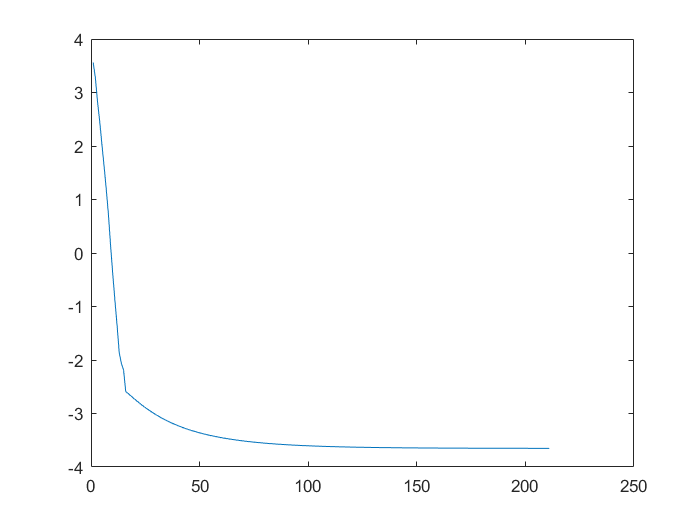
\includegraphics[scale=.3]{../fig/q1_2.png}
	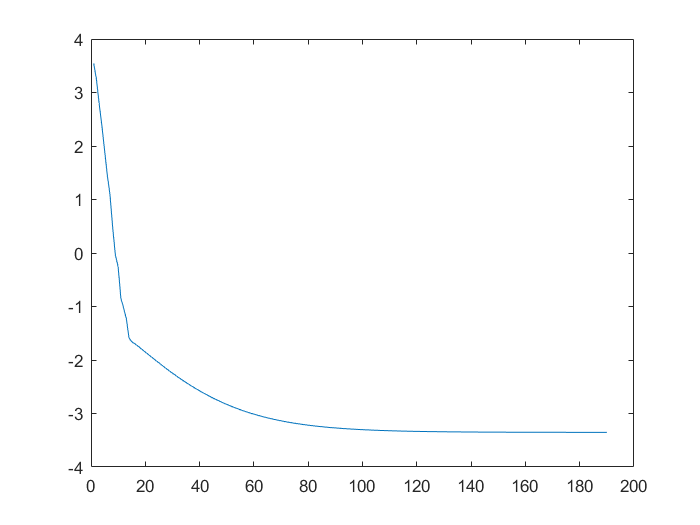
\includegraphics[scale=.3]{../fig/q2_2.png}
	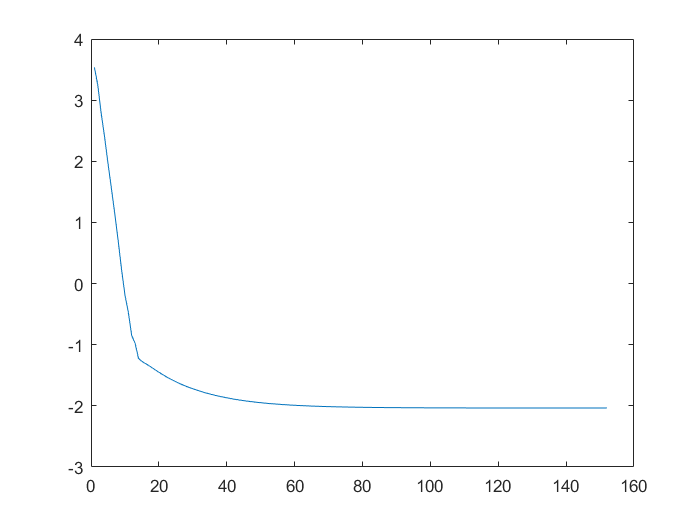
\includegraphics[scale=.3]{../fig/q3_2.png}
\end{figure}
\begin{figure}[H]
	\caption{Convergence History of three problems, x-axis: iter, y-axis: $\log_{10}(\|U-U_0\|_{\infty})$. $h = 1/4$.}
	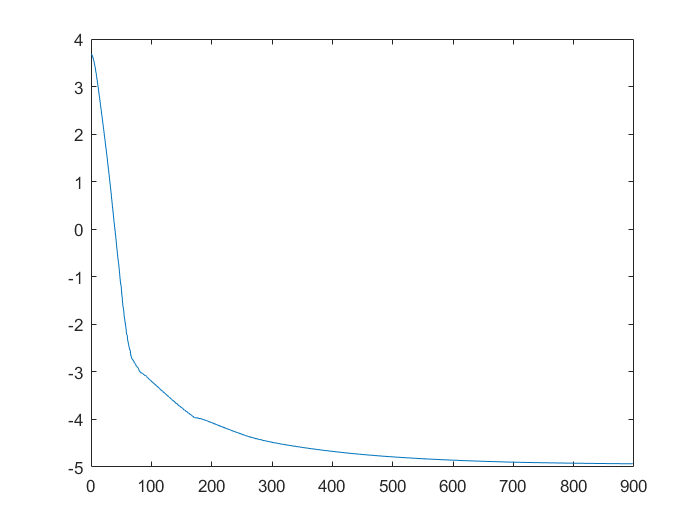
\includegraphics[scale=.3]{../fig/q1_4.png}
	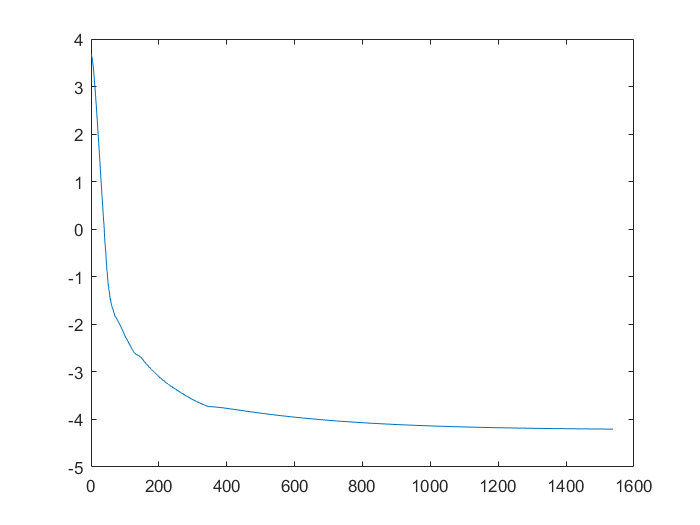
\includegraphics[scale=.3]{../fig/q2_4.png}
	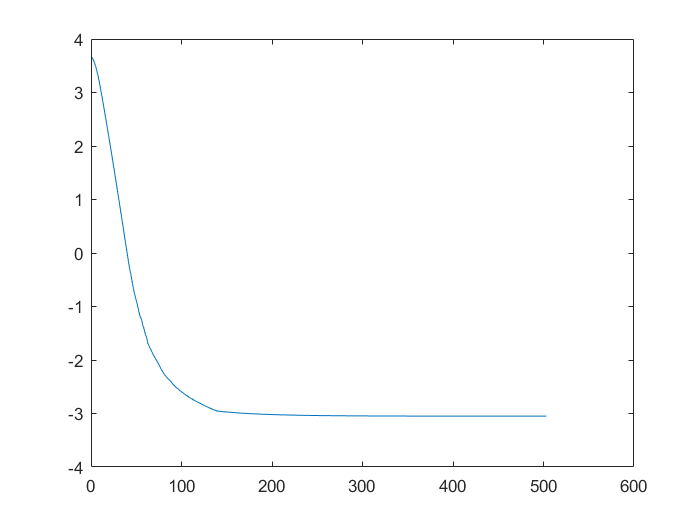
\includegraphics[scale=.3]{../fig/q3_4.png}
\end{figure}

\subsection{Discussion}
When $u$ is smooth enough, we can observe the second order convergence, both $W_p^2$ and $L_{\infty}$ norm. But when $u$ is piecewise smooth or singular, the order cannot be observed so clearly. 

Also, the error seems heavily dependent on the numerical integration, as we see in the table. Early stop will not damage the structure. 

In experiment, the induced mesh will change usually reflects a big decreases of error. (In the figures above, mesh only changes in first circa 1/10 iterations.) This may enlighten us to develop an accelerated version of Perron's iteration, either using parallel techniques or using a nonlinear solver. 
\end{document}





Escape special TeX symbols (%, &, _, #, $)